\documentclass[12pt,compress,english,utf8,t]{beamer}

\usepackage{etex}

\usepackage[english]{babel}

\usepackage{tikz}
\usepackage{booktabs}
\usepackage{ragged2e}
\usepackage{mathtools}

\usetikzlibrary{calc,shapes.callouts,shapes.arrows}
\definecolor{darkred}{RGB}{220,0,0}
\newcommand{\hcancel}[5]{%
    \tikz[baseline=(tocancel.base)]{
        \node[inner sep=0pt,outer sep=0pt] (tocancel) {#1};
        \draw[darkred, line width=1mm] ($(tocancel.south west)+(#2,#3)$) -- ($(tocancel.north east)+(#4,#5)$);
    }%
}%

\usepackage[protrusion=true,expansion=true]{microtype}

\title{The secret of the number 5}
\author{Ingo Blechschmidt}
\institute{32th Chaos Communication Congress}
\date{December 28th, 2015}

\usetheme{Warsaw}
\usecolortheme{seahorse}
\definecolor{mypurple}{RGB}{60,0,255}
\setbeamercolor{structure}{fg=mypurple}
\usefonttheme{serif}
\usepackage[T1]{fontenc}
\usepackage{libertine}
\useinnertheme{rectangles}
\setbeamercovered{invisible}

\setbeamertemplate{title page}[default][colsep=-1bp,rounded=false,shadow=false]
\setbeamertemplate{frametitle}[default][colsep=-2bp,rounded=false,shadow=false,center]

\setbeamertemplate{navigation symbols}{}
\setbeamertemplate{headline}{}

\newcommand*\oldmacro{}%
\let\oldmacro\insertshorttitle%
\renewcommand*\insertshorttitle{%
  \oldmacro\hfill\insertframenumber\,/\,\inserttotalframenumber\hfill}

\newcommand{\defeq}{\vcentcolon=}

\newcommand{\hil}[1]{{\usebeamercolor[fg]{item}{\textbf{#1}}}}

\newcommand{\atpos}[1]{%
  \begin{tikzpicture}[remember picture, overlay]%
    \node[anchor=south east] at (current page.south east) {#1};
  \end{tikzpicture}%
}

\newcommand{\centeredpar}[2]{%
  \begin{center}
    \colorbox{white}{\parbox{#1\textwidth}{%
      #2%
    }}%
  \end{center}%
}

\newcommand{\icfrac}[4]{#1 + \dfrac{1}{#2 + \dfrac{1}{#3 + \dfrac{1}{#4 + \ddots}}}}
\newcommand{\icfracc}[3]{\dfrac{1}{#1 + \dfrac{1}{#2 + \dfrac{1}{#3 + \ddots}}}}
\newcommand{\icfraccc}[2]{\dfrac{1}{#1 + \dfrac{1}{#2 + \ddots}}}

% Gonzalo Medina, http://tex.stackexchange.com/a/228198
\makeatletter
\def\Mdescription#1{%
  \advance\beamer@descdefault by \labelsep%
  \list
  {}
  {\labelwidth\beamer@descdefault%
  \leftmargin\beamer@descdefault%
  \let\makelabel\beamer@descriptionitem
  \settowidth\labelwidth{\beamer@descriptionitem{#1}}%
  \setlength\leftmargin{\labelwidth}% 
  \addtolength\leftmargin{\labelsep}%
  }%
  \beamer@cramped%
  \raggedright
  \beamer@firstlineitemizeunskip%
}
\def\endMdescription{\ifhmode\unskip\fi\endlist}
\long\def\beamer@descriptionitem#1{%
  \def\insertdescriptionitem{#1}%
  {\usebeamertemplate**{description item}}\hfil}
\makeatother

\setbeameroption{show notes}
\setbeamertemplate{note page}[plain]

\begin{document}

\frame{
  \titlepage

  \vspace*{-2em}
  \begin{center}
    \small
    \emph{Watch this space for details on the talk.}
    \medskip

    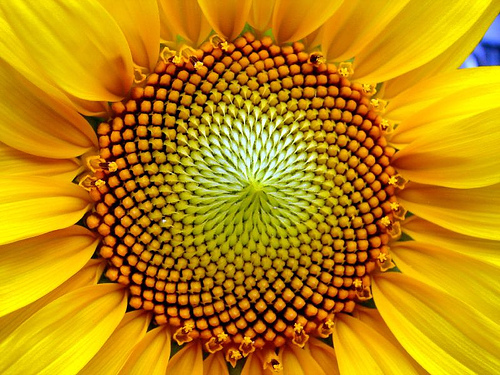
\includegraphics[height=0.25\textheight]{sonnenblume}\quad
    
\includegraphics[height=0.25\textheight]{mandelbrot}\quad
    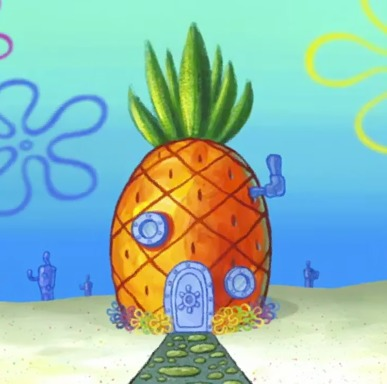
\includegraphics[height=0.25\textheight]{spongebob-ananas}
  \end{center}
}

% http://joachim-reichel.org/software/fraktal/mandelbrot_large.png

\section{A design pattern in nature}

\begin{frame}\frametitle{A design pattern in nature}
  \begin{center}
    \includegraphics[height=0.8\textheight]{mat/21253165_l}
    % 34 counterclockwise, 21 clockwise

    %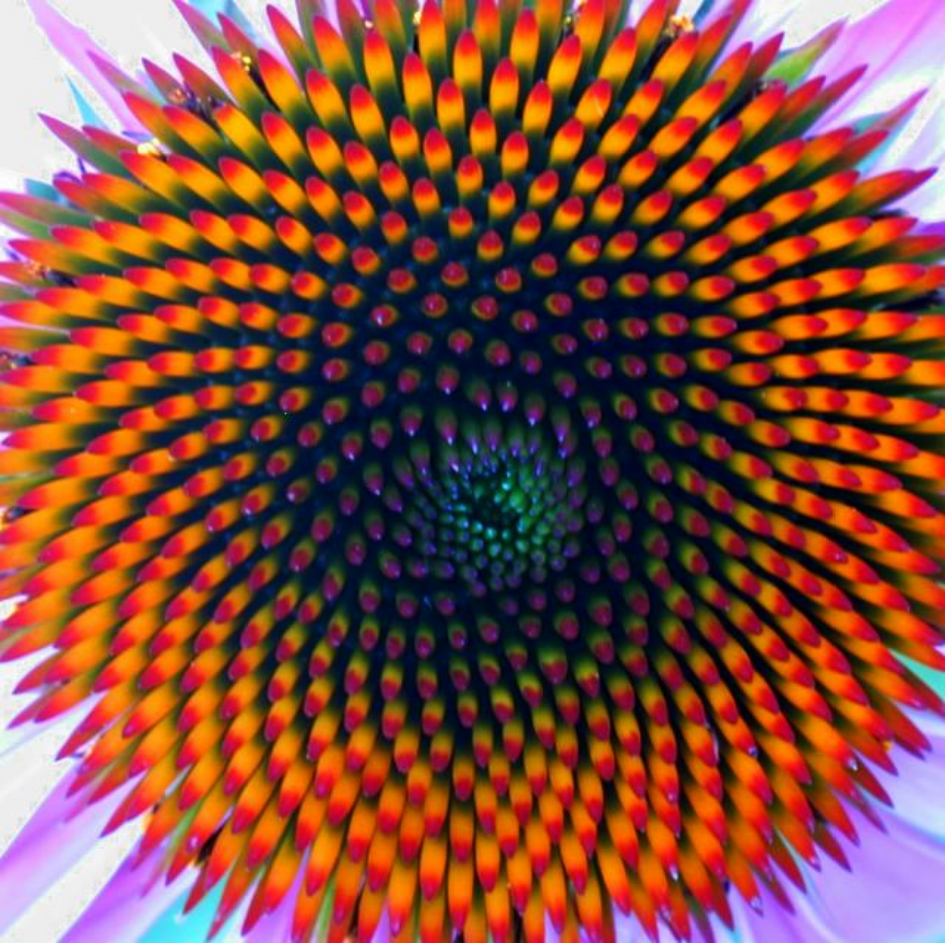
\includegraphics[height=0.8\textheight]{mat/blume}
  \end{center}
\end{frame}


\section{Continued fractions}

\subsection{Examples}

\begin{frame}\frametitle{A curious fraction}
  \only<2-3>{\vspace*{-1em}}
  \only<1>{\Huge}
  \only<1-3>{\[
    \icfrac{1}{2}{2}{2} = {?}
  \]}
  \only<2-3>{\vspace*{1em}}

  \pause
  Crucial observation: Setting
  \only<1-3>{\[ x \defeq {?} - 1 = \icfracc{2}{2}{2}, \]}
  \only<4->{\[ x \defeq {?} - 1 = \icfraccc{2}{2}, \]}
  \pause
  there is the identity
  \[ \frac{1}{2 + x} = x. \]
  \pause
  \pause

  Multiplying by the denominator, we obtain
  \only<5>{$1 = x \cdot (2 + x),$}%
  \only<6->{$1 = 2x + x^2,$}
  \pause
  \pause
  so we only have to solve the quadratic equation
  $0 = x^2 + 2x - 1,$
  \pause
  thus
  \[ x = \frac{-2 + \sqrt{8}}{2} = -1 + \sqrt{2}
    \quad\text{or}\quad
     x = \frac{-2 - \sqrt{8}}{2} = -1 - \sqrt{2}. \]
  It's the positive possibility.
\end{frame}

\begin{frame}\frametitle{More examples}
  \only<1-2>{\vspace*{-2em}\begin{align*}
    \visible<2>{[1; 2, 2, 2, \ldots] =} \icfrac{1}{2}{2}{2} &= \sqrt{2} \\[1.5em]
    \visible<2>{[2; 4, 4, 4, \ldots] =} \icfrac{2}{4}{4}{4} &= \sqrt{5} \\[1.5em]
    \visible<2>{[3; 6, 6, 6, \ldots] =} \icfrac{3}{6}{6}{6} &= \sqrt{10}
  \end{align*}}

  \pause
  \pause

  \begin{enumerate}
    \item $\phantom{0}\sqrt{2} = [1; 2, 2, 2, 2, 2, 2, \ldots]$
    \item $\phantom{0}\sqrt{5} = [2; 4, 4, 4, 4, 4, 4, \ldots]$
    \item $\sqrt{10} = [3; 6, 6, 6, 6, 6, 6, \ldots]$
    \item $\phantom{0}\sqrt{6} = [2; 2, 4, 2, 4, 2, 4, \ldots]$
    \item $\sqrt{14} = [3; 1, 2, 1, 6, 1, 2, \ldots]$
  \end{enumerate}
\end{frame}

\begin{frame}\frametitle{The Euclidean algorithm}
  Recall $\sqrt{2} = [1; 2, 2, 2, \ldots] = 1{,}41421356\ldots$
  \begin{align*}
    1{,}41421356\ldots &= 1 \cdot 1{,}00000000\ldots + 0{,}41421356\ldots \\
    1{,}00000000\ldots &= 2 \cdot 0{,}41421356\ldots + 0{,}17157287\ldots \\
    0{,}41421356\ldots &= 2 \cdot 0{,}17157287\ldots + 0{,}07106781\ldots \\
    0{,}17157287\ldots &= 2 \cdot 0{,}07106781\ldots + 0{,}02943725\ldots \\
    0{,}07106781\ldots &= 2 \cdot 0{,}02943725\ldots + 0{,}01219330\ldots \\
    0{,}02943725\ldots &= 2 \cdot 0{,}01219330\ldots + 0{,}00505063\ldots \\
    &\,\,\,\vdots
  \end{align*}
\end{frame}

\begin{frame}\frametitle{Best approximations using continued fractions}
  \textbf{Theorem.} Cutting off the infinite fraction expansion of a number~$x$
  yields a fraction $a/b$ which is closest to~$x$ under all fractions with
  denominator~$\leq b$.
  \medskip
  \pause

  \textbf{Bonus.} The approximation~$a/b$ is % XXX umso
  better % XXX je größer der nächste Koeffizient in der Entwicklung ist.
\end{frame}


\end{document}

Plan of the talk:

1. Images of spirals in nature; notice Fibonacci numbers.
2. Infinite continued fraction:
   * Example with [1; 2, ...]
   * More examples (only listed)
   * Euclidean algorithm (with illustration?)
   * Theorem about best approximation
3. Approximation of pi
   * List original sources for 22/7 and 355/113
   * Explain using continued fractions
4. Spirals in nature
   * angle, need "most irrational number"
   * golden ratio (also explain as a ratio)
   * simulations
5. Fibonacci numbers in the Mandelbrot fractal
6. Vi Hart

Mention rational tangles?
